%Generazione delle variabili che andranno a sostituire quelle del template 'HomePage.tex'
\newcommand{\documento}{\PdQ}
\newcommand{\nomedocumentofisico}{PianoDiQualifica.pdf}
\newcommand{\redazione}{\MP\\ & \MV}
\newcommand{\verifica}{\SM}
\newcommand{\approvazione}{\GR}
\newcommand{\uso}{Esterno}
\newcommand{\datacreazione}{12 Dicembre 2015}
\newcommand{\datamodifica}{29 Dicembre 2015}
\newcommand{\stato}{Sviluppo}
\newcommand{\destinateTo}{\TV, \\ & \RC, \\ & \ZU}

\def\TABELLE{false}	%abilita - disabilita l'indice delle tabelle
\def\FIGURE{false} 	%abilita - disabilita l'indice delle figure

\documentclass[a4paper,11pt]{article}

%***IMPORTAZIONE PACKAGE***
\usepackage{ifthen}
\usepackage[italian]{babel}
\usepackage[utf8]{inputenc}
\usepackage[T1]{fontenc}
\usepackage{float}
\usepackage{chapterbib}
\usepackage{graphicx}
\usepackage[a4paper,top=2.5cm,bottom=2.5cm,left=2.5cm,right=2.5cm]{geometry}
\usepackage[colorlinks=true, urlcolor=black, citecolor=black, linkcolor=black]{hyperref}
\usepackage{booktabs}
\usepackage{fancyhdr}
\usepackage{totpages}
\usepackage{tabularx, array}
\usepackage{dcolumn}
\usepackage{epstopdf}
\usepackage{booktabs}
\usepackage{fancyhdr}
\usepackage{longtable}
\usepackage{calc}
\usepackage{datatool}
\usepackage[bottom]{footmisc}
\usepackage{listings} 
\usepackage{textcomp}
\usepackage{titlesec}
\usepackage{rotating} 
\usepackage{multirow}
\usepackage{placeins}
\usepackage{color}
\usepackage[table,usenames,dvipsnames]{xcolor}
\usepackage{hyperref}
\usepackage{makecell}
\usepackage{hyperref}


%***STILE PAGINA***
\pagestyle{fancy}
%no indentazione paragrafo
\setlength{\parindent}{0pt}

%***INTESTAZIONE***
\lhead{\Large{\progetto} \\ \footnotesize{\documento}}
\rhead{
\includegraphics[keepaspectratio = true, width = 25px] {../../Template/icone/LogoGruppo.png}}
\renewcommand{\headrulewidth}{0.4pt}  %Linea sotto l'intestazione

%***PIÈ DI PAGINA***
\lfoot{\textit{\gruppoLink}\\ \footnotesize{\email}}
\rfoot{\thepage} %per le prime pagine: mostra solo il numero romano
\cfoot{}
\renewcommand{\footrulewidth}{0.4pt}   %Linea sopra il piè di pagina

%***INSERIMENTO DI NUOVE SOTTOSEZIONI
\setcounter{secnumdepth}{7}		% mostra nel documento fino al livello 8 (1.2.3.4.5.6.7.8)
\setcounter{tocdepth}{7}			% mostra nell'indice fino al livello 8 (1.2.3.4.5.6.7.8)

%***LA SOTTOSEZIONE PARAGRAPH VIENE VISUALIZZATA COME UNA SECTION
\titleformat{\paragraph}{\normalfont\normalsize\bfseries}{\theparagraph}{1em}{}
\titlespacing*{\paragraph}{0pt}{3.25ex plus 1ex minus .2ex}{1.5ex plus .2ex}

\titleformat{\subparagraph}{\normalfont\normalsize\bfseries}{\thesubparagraph}{1em}{}
\titlespacing*{\subparagraph}{0pt}{3.25ex plus 1ex minus .2ex}{1.5ex plus .2ex}

\makeatletter
\newcounter{subsubparagraph}[subparagraph]
\renewcommand\thesubsubparagraph{%
  \thesubparagraph.\@arabic\c@subsubparagraph}
\newcommand\subsubparagraph{%
  \@startsection{subsubparagraph}    % counter
    {6}                              % level
    {\parindent}                     % indent
    {3.25ex \@plus 1ex \@minus .2ex} % beforeskip
    {0.75em}                           % afterskip
    {\normalfont\normalsize\bfseries}}
\newcommand\l@subsubparagraph{\@dottedtocline{6}{10em}{5.5em}} %gestione dell'indice
\newcommand{\subsubparagraphmark}[1]{}
\makeatother

\makeatletter
\newcounter{subsubsubparagraph}[subsubparagraph]
\renewcommand\thesubsubsubparagraph{%
  \thesubsubparagraph.\@arabic\c@subsubsubparagraph}
\newcommand\subsubsubparagraph{%
  \@startsection{subsubsubparagraph}    % counter
    {7}                              % level
    {\parindent}                     % indent
    {3.25ex \@plus 1ex \@minus .2ex} % beforeskip
    {0.75em}                           % afterskip
    {\normalfont\normalsize\bfseries}}
\newcommand\l@subsubsubparagraph{\@dottedtocline{7}{10em}{6.5em}} %gestione dell'indice
\newcommand{\subsubsubparagraphmark}[1]{}
\makeatother
%Generali
\newcommand{\progetto}{QuizziPedia}
\newcommand{\gruppo}{TheFellowshipOfTheCode}
\newcommand{\gruppoLink}{\href{http://thefellowshipofthecode.github.io/}{TheFellowshipOfTheCode}}
\newcommand{\email}{\href{mailto:thefellowshipofthecode@gmail.com}{thefellowshipofthecode@gmail.com}}

%Documenti
\newcommand{\AdR}{Analisi dei Requisiti}
\newcommand{\NdP}{Norme di Progetto}
\newcommand{\PdP}{Piano di Progetto}
\newcommand{\SdF}{Studio di Fattibilità}
\newcommand{\PdQ}{Piano di Qualifica}
\newcommand{\VI}{Verbale Interno}
\newcommand{\VE}{Verbale Esterno}
\newcommand{\ST}{Specifica Tecnica}
\newcommand{\DDP}{Definizione di Prodotto}
\newcommand{\MU}{Manuale Utente}
\newcommand{\G}{Glossario}
\newcommand{\LdP}{Lettera di Presentazione}
\newcommand{\NdPv}{NormeDiProgetto\_v\_1\_0\_0}
\newcommand{\PdPv}{PianoDiProgetto\_v\_1\_0\_0}
\newcommand{\PdQv}{PianoDiQualifica\_v\_1\_0\_0}
\newcommand{\SdFv}{StudioDiFattibilità\_v\_1\_0\_0}

%Componenti del gruppo
\newcommand{\AF}{Alberto Ferrara}
\newcommand{\SM}{Simone Magagna}
\newcommand{\FB}{Franco Berton}
\newcommand{\MP}{Marco Prelaz}
\newcommand{\MV}{Mattia Varotto}
\newcommand{\GN}{Matteo Gnoato}
\newcommand{\GR}{Matteo Granzotto}

%Ruoli
\newcommand{\RdP}{Responsabile di Progetto}
\newcommand{\Res}{Responsabile}
\newcommand{\Amm}{Amministratore}
\newcommand{\Ver}{Verificatore}
\newcommand{\Prog}{Progettista}
\newcommand{\Progr}{Programmatore}
\newcommand{\Ana}{Analista}
\newcommand{\RdPs}{Responsabili di Progetto}
\newcommand{\Ress}{Responsabile}
\newcommand{\Amms}{Amministratori}
\newcommand{\Vers}{Verificatori}
\newcommand{\Progs}{Progettisti}
\newcommand{\Progrs}{Programmatori}
\newcommand{\Anas}{Analisti}

%Professori e proponente
\newcommand{\TV}{Prof. Tullio Vardanega}
\newcommand{\RC}{Prof. Riccardo Cardin}
\newcommand{\ZU}{Zucchetti S.P.A.}
\newcommand{\proponente}{Zucchetti S.P.A.}

\newcommand{\diaryEntry}[5]{#2 & \emph{#4} & #3 & #5 & #1\\ \hline}

%comando per una nuova riga nella tabella del diario delle modifiche
\newcommand{\specialcell}[2][c]{%
	\begin{tabular}[#1]{@{}c@{}}#2\end{tabular}}

\renewcommand*\sectionmark[1]{\markboth{#1}{}}
\renewcommand*\subsectionmark[1]{\markright{#1}}

%Pediodi di lavoro 
\newcommand{\AR}{Analisi dei Requisiti}
\newcommand{\AD}{Analisi dei Requisiti in Dettaglio}
\newcommand{\PA}{Progettazione Architetturale}
\newcommand{\PD}{Progettazione di Dettaglio}
\newcommand{\CO}{Codifica}
\newcommand{\VV}{Verifica e Validazione}

% Revisioni
\newcommand{\RR}{Revisione dei Requisiti}
\newcommand{\RP}{Revisione di Progettazione}
\newcommand{\RQ}{Revisione di Qualifica}
\newcommand{\RA}{Revisione di Accettazione}

% Comandi analisi dei requisiti
\newcommand{\uau}{utente autenticato}
\newcommand{\uaus}{utenti autenticati}
\newcommand{\uaupro}{utente autenticato pro}
\newcommand{\uauspro}{utenti autenticati pro}

\newcommand{\myincludegraphics}[2][]{%
	\setbox0=\hbox{\phantom{X}}%
	\vtop{
		\hbox{\phantom{X}}
		\vskip-\ht0
		\hbox{\includegraphics[#1]{#2}}}}
\newcommand{\modificheuno} 
{	
	0.0.3 & Inseriti i primi riferimenti informativi & \specialcell[t]{\GN \\ \prog} & 2016-02-26
	\\\midrule
	0.0.2 & Stesura scopo del documento, scopo del prodotto , riferimenti normativi & \specialcell[t]{\GN \\ \prog} & 2016-02-26
	\\\midrule
	0.0.1 & Creato template documento & \specialcell[t]{\GN \\ \prog} & 2016-02-26
	\\\midrule
}
\newcommand{\modifichedue}
{
}
\begin{document}

%inclusione template HomePage
\begin{center}

%
\includegraphics[width=1em]{../../../Template/icone/LogoGruppo.png}
\begin{large} \textbf{\gruppoLink} \end{large}
%
\includegraphics[width=1em]{../../../Template/icone/LogoGruppo.png}
\vspace{0.2em}

\hrule
\vspace{3em}


\includegraphics[keepaspectratio = true, width=8cm]{../../../Template/icone/LogoGruppo.png}

%Prima pagina senza intestazione né piè di pagina	
\thispagestyle{empty}

%Le informazioni del documento sono ancorate a fine pagina
\vfill

%Copertina
\begin{center} 
  \begin{Huge}
  {\fontsize{15mm}{20mm}\selectfont \progetto} 
  \end{Huge}
\end{center}

\begin{Huge} \documento \end{Huge}

\begin{center}
\textbf{Informazioni sul documento} \\ \vspace{2em}
\small
\begin{tabular}{r|l}
	\textbf{Nome Documento} & \nomedocumentofisico \\
	\textbf{Versione}	& 1\\
	\textbf{Data di Creazione} & \datacreazione\\
	\textbf{Data ultima modifica} & \datamodifica\\
	\textbf{Stato} & \stato \\
	\textbf{Redazione}	& \redazione\\
	\textbf{Verifica}	& \verifica\\
	\textbf{Approvazione}	& \approvazione\\
	\textbf{Uso}  & \uso\\
	\textbf{Distribuzione} & \gruppo \\
	\textbf{Destinato a}  &  \destinateTo \\
	\textbf{Email di riferimento} & \email
\end{tabular}
\end{center}

\normalsize
%Sommario
\textbf{Sommario\\} 
Documento contenente le norme di progetto che il gruppo \textit{\gruppo} seguirà durante tutte le fasi di realizzazione del prodotto \textit{\progetto}.

%\vfill %cosa fa?
\end{center}
\clearpage

\newpage
%***REGISTRO DELLE MODIFICHE***
%Vari comandi per la struttura della tabella, NON MODIFICARE!
\begin{center}
	\Large{\textbf{Registro delle modifiche}}
	\\\vspace{0.5cm}
	\normalsize
	\begin{tabularx}{\textwidth}{cXcc}
		\textbf{Versione} & \textbf{Descrizione} & \textbf{Autore e Ruolo} & \textbf{Data} \\\toprule
		\modifiche
		\bottomrule
\end{tabularx}
\end{center}
\newpage
\tableofcontents
%sezioni documento

\newpage
\section{Introduzione}

\subsection{Scopo del documento}
Il presente documento ha lo scopo di definire in dettaglio la struttura e il funzionamento delle componenti del progetto \progetto. Questo documento servirà come guida per i \textit{\Progrs} del gruppo \gruppo fornendo direttive e vincoli per la realizzazione del \textit{progetto\ped{G}}.

\subsection{Scopo del prodotto}
Lo scopo del prodotto è di permettere la creazione e gestione di questionari in grado di identificare le lacune dei candidati prima, durante e al termine di un corso di formazione. 
\\Il sistema dovrà offrire le seguenti funzionalità:
\begin{itemize}
	\item
	Archiviare questionari in un server suddivisi per argomento;
	\item
	Somministrare all'utente, tramite un'interfaccia, questionari specifici per argomento scelto;
	\item
	Verificare e valutare i questionari scelti dagli utenti in base alle risposte date.
\end{itemize}
La parte destinata ai creatori di questionari dovrà essere fruibile attraverso un \textit{browser\ped{G}} desktop, abilitato all'utilizzo delle tecnologie \textit{HTML5\ped{G}}, \textit{CSS3\ped{G}} e \textit{JavaScript\ped{G}}. La parte destinata agli esaminandi sarà utilizzabile su qualunque dispositivo: dal personal computer ai tablet e smartphone.

\subsection{Glossario}
Al fine di evitare ogni ambiguità i termini tecnici del dominio del progetto, gli acronimi e le parole che necessitano di ulteriori spiegazioni saranno nei vari documenti marcate con il pedice \ped{G} e quindi presenti nel documento \textit{\G}.


\subsection{Riferimenti}
\subsubsection{Normativi}
\begin{itemize}
	\item \textit{\NdPv};
	\item \textit{\AdRvDue};
\end{itemize}
\subsubsection{Informativi}
\begin{itemize}
	\item \textbf{Ingegneria del software - Ian Sommerville - 8a edizione (2007)}: \\
	Parte terza: Progettazione, capitolo 11: Progettazione architetturale, Capitolo 14: Progettazione orientata agli oggetti;
	\item \textbf{Design Patterns} - Erich Gamma, Richard Helm, Ralph Johnson, John Vlissides - 1a edizione italiana (2006);
	\item \textbf{Slide dell'insegnamento - Design patterns:}
	\begin{itemize}
		\item Strutturali: \url{http://www.math.unipd.it/~tullio/IS-1/2015/Dispense/E07.pdf};
		\item Creazionali: \url{http://www.math.unipd.it/~tullio/IS-1/2015/Dispense/E08.pdf}
		\item Comportamentali: \url{http://www.math.unipd.it/~tullio/IS-1/2015/Dispense/E09.pdf}
		\item Architetturali:
			\begin{itemize}
				\item \url{http://www.math.unipd.it/~rcardin/sweb/Design%20Pattern%20Architetturali%20-%20Model%20View%20Controller_4x4.pdf};
				\item \url{http://www.math.unipd.it/~rcardin/sweb/Design%20Pattern%20Architetturali%20-%20Dependency%20Injection_4x4.pdf}.
			\end{itemize} 
	\end{itemize}
	\item \textbf{Martin Fowler - UML\ped{G} Distilled} - 2nd edition;
	\item \textbf{Slide dell'insegnamento - Diagrammi delle classi}: \\
		\url{http://www.math.unipd.it/~tullio/IS-1/2015/Dispense/E03.pdf}
	\item \textbf{Slide dell'insegnamento - Diagrammi dei packages:} \\
		\url{http://www.math.unipd.it/~tullio/IS-1/2015/Dispense/E04.pdf}
	\item \textbf{Slide dell'insegnamento - Diagrammi di sequenza:} \\
		\url{http://www.math.unipd.it/~tullio/IS-1/2015/Dispense/E05.pdf}
	\item \textbf{Documentazione del \textit{Framework\ped{G}MEAN\ped{G}.js}:} \\
		\url{http://learn.mean.io/}
	\item \textbf{Documentazione della \textit{piattaforma} Node.js:} \\
		\url{https://nodejs.org/api/}
	\item \textbf{Giuda all'utilizzo dei middleware Express:} \\
		\url{http://expressjs.com/it/guide/using-middleware.html}
	\item \textbf{Guida all'utilizzo dei middleware Passport:} \\
		\url{http://passportjs.org/docs}
	\item \textbf{Manuale del database \textit{MongoDB\ped{G}}:} \\
		\url{https://docs.mongodb.org/manual/}
	\item \textbf{Documentazione dell'interfaccia REST:}
		\begin{itemize}
			\item \textit{Descrizione di REST:} \url{https://it.wikipedia.org/wiki/Representational_State_Transfer}
			\item \textit{Descrizione risorse REST:} \url{http://stashboard.readthedocs.org/en/latest/restapi.html}
		\end{itemize}
	\item \textbf{Documentazione del \textit{framework\ped{G} AngularJS\ped{G}}:} \\
		\begin{itemize}
			\item \textit{Documentazione generica:} \url{https://docs.angularjs.org/guide}
			\item \textit{Documentazione servizio \$http:} \url{https://docs.angularjs.org/api/ng/service/\$http}
			\item \textit{Documentazione servizio \$location:} \url{https://docs.angularjs.org/api/ng/service/\$location}
			\item \textit{Documentazione servizio \$windows:} \url{https://docs.angularjs.org/api/ng/service/\$window}
			\item \textit{Documentazione servizio \$ruoteParams:} \url{https://docs.angularjs.org/api/ngRoute/service/\$routeParams}
			\item \textit{Documentazione servizio \$q:} \url{https://docs.angularjs.org/api/ng/service/\$q}
		\end{itemize}
	\item \textbf{Documentazione del \textit{framework\ped{G}} Material for Angular:} \\
		\url{https://material.angularjs.org/latest/}
	\item \textbf{Documentazione del \textit{framework\ped{G}} Chart.js} \\
		\url{http://www.chartjs.org/docs/}
	\item \textbf{Documentazione del \textit{wrapper\ped{G}} Angles.js} \\
		\url{https://github.com/gonewandering/angles}
	\item \textbf{Documentazione del \textit{framework\ped{G}} TextAngular.js} \\
		\url{https://github.com/fraywing/textAngular/wiki/textAngular-Docs-v1.1.x}
	\item \textbf{Guida all'utilizzo della direttiva \textit{ng-file-upload}} \\
		\url{https://github.com/danialfarid/ng-file-upload}
	\item \textbf{Documentazione di \textit{jison\ped{G}} per la definizione della grammatica di QML} \\
		\url{http://zaa.ch/jison/docs/}
\end{itemize}
\newpage
\section{Strategie di verifica}
\subsection{Definizione degli obiettivi}
\subsubsection{Standard per la qualità di processo}
Per garantire la qualità del prodotto è necessario perseguire la qualità dei processi che lo definiscono. Per fare ciò si è deciso di adottare lo standard \textit{ISO/IEC 15504\ped{G}} denominato \textit{SPICE\ped{G}} il quale fornisce gli strumenti necessari a valutare la qualità di questi ultimi.\\
Per applicare correttamente questo modello si deve utilizzare il ciclo \textit{PDCA\ped{G}} che definisce una metodologia di controllo dei processi durante il loro ciclo di vita e che consente di migliorarne in modo continuativo la qualità.

\subsubsection{Standard per la qualità di prodotto}
Al fine di aumentare il valore commerciale di un prodotto software e di garantirne il corretto funzionamento è necessario fissare degli obiettivi qualitativi e di assicurare che questi vengano effettivamente rispettati.\\
Lo standard \textit{ISO/IEC 9126\ped{G}} è stato redatto con lo scopo di descrivere questi obiettivi e delineare delle metriche capaci di misurare il raggiungimento di tali obiettivi.

\subsection{Procedure per il controllo della qualità di processo}
La qualità dei processi sarà garantita dall'applicazione del principio \textit{PDCA\ped{G}}, descritto nell'appendice A. Così facendo, sarà possibile garantire un miglioramento continuo della qualità di tutti i processi, inclusa la verifica, ottenendo di conseguenza il miglioramento dei prodotti risultanti.\\
Per avere controllo sulla qualità è necessario che:
\begin{itemize}
\item I processi siano pianificati nel dettaglio;
\item Nella pianificazione siano ripartite in modo chiaro le risorse;
\item I processi vengano costantemente monitorati.
\end{itemize}
L'attuazione di tali punti è descritta dettagliatamente nel \textit{\PdP}.\\
La qualità dei processi viene inoltre monitorata mediante l'analisi costante della qualità del prodotto e quantificata utilizzando varie metriche, descritte nella sezione 2.9.1. Un prodotto di bassa qualità indica un processo da migliorare.

\subsection{Procedure per il controllo della qualità di prodotto}
Il controllo di qualità del prodotto verrà garantito da:
\begin{itemize}
\item \textbf{\textit{Quality Assurance\ped{G}}}: insieme di attività realizzate per garantire il raggiungimento degli obiettivi di qualità. Prevede l'attuazione di tecniche di analisi statica e dinamica, descritte nella sezione 2.8;
\item \textbf{Verifica}: processo che determina se l'output di una fase è consistente, completo e corretto. La verifica andrà eseguita costantemente durante l'intera durata del progetto;
\item \textbf{Validazione}: conferma in modo oggettivo che il sistema risponda ai requisiti.
\end{itemize}

\subsection{Organizzazione}
L'organizzazione della strategia di verifica si basa sull'attuazione di attività di verifica per ogni processo attuato. Per ogni processo realizzato viene verificata la qualità del processo stesso e la qualità dell'eventuale prodotto ottenuto da esso.\\
Ognuna delle fasi di progetto descritte nel \textit{\PdP} necessita di diverse attività di verifica a causa della differente natura degli output ottenuti.\\
Essendo la redazione dei documenti un'attività predominante e costantemente presente nel progredire del progetto, il processo di verifica si suddividerà in due attività per garantirne una maggiore qualità: Analisi e Analisi di Dettaglio. In ogni documento viene inoltre incluso il diario delle modifiche che permette di mantenere uno storico delle attività svolte e delle relative responsabilità.

\subsection{Pianificazione strategica e temporale}
Avendo l'obiettivo di rispettare le scadenze fissate nel \textit{\PdP}, è necessario che l'attività di verifica della documentazione sia sistematica e ben organizzata. Procedendo in questo modo, l'individuazione e la correzione di eventuali errori avverrà il prima possibile, impedendo una loro rapida diffusione. Ogni attività di redazione dei documenti e di codifica deve essere preceduta da uno studio preliminare sulla struttura e sui contenuti degli stessi con lo scopo di ridurre la possibilità di commettere imprecisioni di natura concettuale e tecnica favorendo quindi l'attività di verifica, dove saranno necessari minori interventi di correzione.

\subsection{Responsabilità}
Per garantire che il processo di verifica sia efficace e sistematico vengono attribuite delle responsabilità a degli specifici ruoli di progetto.\\
I ruoli che detengono le responsabilità del processo di verifica sono il \textit{\RdP} ed i \textit{\Vers}. La suddivisione dei compiti e le modalità di attuazione degli stessi sono definiti nelle \textit{\NdP}.

\subsection{Risorse}
Per assicurare che gli obiettivi qualitativi vengano raggiunti è necessario l'utilizzo di risorse sia umane che tecnologiche. Coloro che detengono la responsabilità maggiore per l'attività di verifica e validazione sono il \textit{\RdP} e il \textit{\Ver}.\\
Per risorse tecniche e tecnologiche sono da intendersi tutti gli strumenti software e hardware che il gruppo intende utilizzare per attuare le attività di verifica su processi e prodotti. Per agevolare il lavoro dei \textit{\Vers} sono stati impiegati numerosi strumenti automatici che eseguono controlli sistematici sui prodotti generati. Tali strumenti sono descritti nelle \textit{\NdP}.

\subsection{Tecniche di analisi}
\subsubsection{Analisi statica}
L'analisi statica è una tecnica di analisi che permette di effettuare la verifica di quanto prodotto individuando errori ed anomalie, applicabile sia alla documentazione che al codice. Essa può essere svolta in due modi distinti ma complementari.

\paragraph{Walkthrough}
Si svolge effettuando una lettura critica a largo spettro. E' una tecnica che viene utilizzata soprattutto nelle prime attività del progetto, quando ancora non è presente una adeguata esperienza da parte dei membri del gruppo, che permetta di attuare una verifica più mirata e precisa.\\
Con l'utilizzo di questa tecnica, il \textit{\Ver} sarà in grado di stilare una lista di controllo con gli errori più frequenti in modo da favorire il miglioramento di tale attività nelle fasi future.\\
Questa è un'attività onerosa e collaborativa che richiede l'intervento di più persone per essere efficacie ed efficiente. Dopo una prima fase di lettura ed individuazione degli errori, segue una fase di discussione con la finalità di esaminare i difetti riscontrati e di proporre le dovute correzioni. L'ultima fase consiste nel correggere gli errori rilevati nello scrivere un rapporto che elenchi le modifiche effettuate.

\paragraph{Inspection}
Questa tecnica consiste nell'analisi mirata di alcune parti del documento o del codice che sono ritenute fonti maggiori di errore. La \textit{lista di controllo}, che deve essere seguita per svolgere efficacemente questo processo, deve essere redatta anticipatamente ed è frutto dell'esperienza maturata dai verificatori attraverso la tecnica di \textit{Walkthrough\ped{G}}.\\
L'\textit{Inspection\ped{G}} è una strategia più rapida del \textit{Walkthrough\ped{G}} in quanto consente l'analisi di alcune parti dei prodotti ritenute critiche dalla checklist e non necessita della lettura integrale dei documenti in oggetto.\\
Diversamente dal \textit{Walkthrough\ped{G}} tale tecnica viene svolta esclusivamente dai verificatori che dopo aver individuato gli errori procedono alla loro correzione e alla redazione di un rapporto di verifica che tenga traccia del lavoro svolto.

\subsubsection{Analisi dinamica}
L'analisi dinamica si applica solamente al prodotto software e viene svolta durante l'esecuzione del codice mediante l'uso di test predisposti per verificarne il funzionamento e rilevare possibili difetti di implementazione.\\
Affinché tale attività sia utile e generi risultati attendibili è necessario che i test effettuati siano ripetibili: questa caratteristica è fondamentale in quanto solo un test che, dato un certo input, produce sempre lo stesso output su uno specifico ambiente, è capace di riscontrare problemi e verificare la correttezza del prodotto software.\\
Di conseguenza devono essere definiti a priori:
\begin{itemize}
\item \textbf{Ambiente}: consiste sia del sistema hardware che di quello software sui quali è stato pianificato l'utilizzo del prodotto software sviluppato; di essi deve essere specificato uno stato iniziale dal quale poter iniziare ad eseguire i test;
\item \textbf{Specifica}: consiste nel definire quali input sono necessari per l'esecuzione del test e quali devono essere gli output attesi;
\item \textbf{Procedure}: consiste nel definire come devono essere svolti i test, in quale ordine e come devono essere analizzati i risultati ottenuti.
\end{itemize}
Sono definibili 5 diversi tipi di test:
\begin{itemize}
\item \textbf{Test di unità};
\item \textbf{Test di integrazione};
\item \textbf{Test di sistema};
\item \textbf{Test di regressione};
\item \textbf{Test di accettazione}.
\end{itemize}

\paragraph{Test di unità}
Consiste nella verifica di ogni singola unità del prodotto software tramite l'utilizzo di \textit{stub\ped{G}}, \textit{driver\ped{G}} e \textit{logger\ped{G}}.\\
Per unità si intende la più piccola quantità di software che è utile verificare singolarmente e che viene prodotta da un singolo programmatore.\\
Attraverso tali test si vuole verificare il corretto funzionamento dei moduli che compongono l'intero sistema in modo da eliminare possibili errori di implementazione da parte dei programmatori.

\paragraph{Test di integrazione}
Consiste nella verifica dei componenti del sistema che vengono aggiunti incrementalmente al prodotto e si prefigge quindi di analizzare che la combinazione di due o più unità software funzionino come previsto.\\
Questo tipo di test serve ad individuare errori residui nella realizzazione dei singoli moduli, modifiche delle interfacce e comportamenti inaspettati di componenti software preesistenti forniti da terze parti che non si conoscono a fondo.\\
Per effettuare tali test devono essere aggiunte delle componenti fittizie al posto di quelle che non sono ancora state sviluppate, in modo da non influenzare negativamente l'esito dell'analisi.

\paragraph{Test di sistema}
Consiste nella validazione del prodotto software nel momento in cui lo si ritiene giunto ad una versione definitiva.\\
Tale test deve verificare che la copertura dei requisiti software stabilite in fase di Analisi di Dettaglio sia totale.

\paragraph{Test di regressione}
Consiste nell'eseguire nuovamente i test riguardanti le componenti software che hanno subito modifiche, in modo da controllare che i cambiamenti apportati non pregiudichino il funzionamento di componenti che non sono stati aggiornati e che precedentemente non erano soggetti ad errori.\\
Tale operazione è aiutata dal tracciamento, che permette di individuare e ripetere facilmente i test di unità, integrazione ed eventualmente sistema che sono stati potenzialmente influenzati dalla modifica.

\paragraph{Test di accettazione}
E' il collaudo del prodotto software che viene eseguito in presenza del proponente. Se tale collaudo viene superato positivamente si può procedere al rilascio ufficiale del prodotto sviluppato.

\subsection{Misure e metriche}
Il processo di verifica, per essere informativo, deve essere quantificabile. Le misure rilevate dal processo di verifica devono quindi essere basate su metriche stabilite a priori. Le metriche incerte, qualora ce ne fossero, si miglioreranno in modo incrementale. Essendo la natura delle metriche molto variabile, vi possono essere due tipologie di range:
\begin{itemize}
\item \textbf{Accettazione}: valori richiesti affinché il prodotto sia accettato;
\item \textbf{Ottimale}: valori entro cui dovrebbe collocarsi la misurazione. Tale range non è vincolante, ma fortemente consigliato. Scostamenti da tali valori necessitano una verifica approfondita.
\end{itemize}

\subsubsection{Metriche per i processi}
Come metrica per i processi si è scelto di utilizzare indici che ne analizzino i costi e i tempi.\\
Tali indici vengono utilizzati anche per mantenere il controllo sui processi durante il loro svolgimento.

\paragraph{Schedule Variance (SV)}
Indica se si è in linea, in anticipo o in ritardo rispetto la pianificazione temporale delle attività nella \textit{baseline\ped{G}}.\\
E' un indicatore di efficacia.\\
Se $SV > 0$ significa che il gruppo di lavoro sta producendo con maggior velocità rispetto a quanto pianificato, viceversa se negativo.\\
\textbf{Parametri utilizzati}:
\begin{itemize}
\item Range-accettazione: $[\geq-(\textit{costo preventivo fase}\times5\%)]$;
\item Range-ottimale: $[\geq0]$.
\end{itemize}

\paragraph{Budget Variance (BV)}
Indica se alla data corrente si è speso di più o di meno rispetto a quanto pianificato.\\
E' un indicatore che ha un valore contabile e finanziario.\\
Se $BV > 0$ significa che l'attuazione del progetto sta consumando il proprio budget con minor velocità rispetto a quanto pianificato, viceversa se negativo.\\
\textbf{Parametri utilizzati}:
\begin{itemize}
\item Range-accettazione: $[\geq-(\textit{costo preventivo fase}\times10\%)]$;
\item Range-ottimale: $[\geq0]$.
\end{itemize}

\subsubsection{Metriche per i documenti}
Come metrica per i documenti redatti si è scelto di utilizzare l'indice di leggibilità.\\
Vi sono a disposizione molti indici di leggibilità, ma i più importanti sono per la lingua inglese. Si è deciso quindi di adottare un indice di leggibilità per la lingua italiana.

\paragraph{Gulpease}
L'\textit{indice Gulpease\ped{G}} è un indice di leggibilità di un testo tarato sulla lingua italiana.\\
Rispetto ad altri ha il vantaggio di utilizzare la lunghezza delle parole in lettere anziché in sillabe, semplificandone il calcolo automatico. Permette di misurare la complessità dello stile di un documento.\\
L'\textit{indice Gulpease\ped{G}} considera due variabili linguistiche: la lunghezza della parola e la lunghezza della frase rispetto al numero delle lettere.\\
L'indice è calcolato secondo la seguente formula:
\begin{center}
$89+\frac{300\times(\textit{numero delle frasi})-10\times(\textit{numero delle lettere})}{\textit{numero delle parole}}$
\end{center}
I risultati sono compresi tra 0 e 100, dove il valore 100 indica la leggibilità più alta e 0 la leggibilità più bassa. In generale risulta che documenti aventi un indice:
\begin{itemize}
\item Inferiore a 80 sono difficili da leggere per chi ha la licenza elementare;
\item Inferiore a 60 sono difficili da leggere per chi ha la licenza media;
\item Inferiore a 40 sono difficili da leggere per chi ha un diploma superiore.
\end{itemize}
\textbf{Parametri utilizzati}:
\begin{itemize}
\item Range-accettazione: $[40-100]$;
\item Range-ottimale: $[50-100]$.
\end{itemize}

\subsubsection{Metriche per il software}
Per poter perseguire gli obiettivi di qualità software, è auspicabile applicare le metriche che ora verranno descritte.\\
Questa sezione è da comprendersi come una dichiarazione di intenti, che verrà rivista nelle prossime revisioni.

\paragraph{Complessità ciclomatica}
Utilizzata per misurare la complessità di funzioni, moduli, metodi o classi di un programma.\\
La \textit{complessità ciclomatica\ped{G}} è calcolata utilizzando il grafo di controllo di flusso del programma: i nodi del grafo corrispondono a gruppi indivisibili di istruzioni, mentre gli archi connettono due nodi se il secondo gruppo di istruzioni può essere eseguito immediatamente dopo il primo gruppo.\\
Altri valori di  \textit{complessità ciclomatica\ped{G}} implicano una ridotta manutenibilità del codice. Valori bassi di  \textit{complessità ciclomatica\ped{G}} potrebbero però determinare scarsa efficienza dei metodi.\\
Questo parametro è inoltre un indice del carico di lavoro richiesto per il testing. Un modulo con complessità elevata richiede più testing di un modulo a complessità inferiore.\\
Parametri utilizzati:
\begin{itemize}
\item Range-accettazione: $[1-15]$;
\item Range-ottimale: $[1-10]$.
\end{itemize}

\paragraph{Numero di livelli di annidamento}
Rappresenta il numero di livelli di annidamento dei metodi, cioè l'inserimento di una struttura di controllo all'interno di un'altra.\\
Un valore elevato di tale indice implica un'alta complessità ed un basso livello di astrazione del codice.\\
Parametri utilizzati:
\begin{itemize}
\item Range-accettazione: $[1-6]$;
\item Range-ottimale: $[1-3]$.
\end{itemize}

\paragraph{Attributi per classe}
Un numero elevato di attributi interni ad una classe potrebbe evidenziare la necessità di suddividere la classe in più classi da mettere in relazione tra di loro, seguendo il principio dell'\textit{incapsulamento\ped{G}}.\\
Un alto valore di questo attributo indica un possibile errore di progettazione.\\
Parametri utilizzati:
\begin{itemize}
\item Range-accettazione: $[0-16]$;
\item Range-ottimale: $[3-8]$.
\end{itemize}

\paragraph{Numero di parametri per metodo}
Un numero elevato di parametri per un metodo potrebbe evidenziare la necessità di ridurre le funzionalità associate a tale metodo.\\
Un alto valore di questo attributo indica un possibile errore di progettazione.\\
Parametri utilizzati:
\begin{itemize}
\item Range-accettazione: $[0-8]$;
\item Range-ottimale: $[0-4]$.
\end{itemize}

\paragraph{Linee di codice per linee di commento}
Indica il rapporto tra linee di codice e linee di commento.\\
E' utile per stimare la manutenibilità del codice.\\
Parametri utilizzati:
\begin{itemize}
\item Range-accettazione: $[>0.25]$;
\item Range-ottimale: $[>0.30]$.
\end{itemize}

\paragraph{Flusso di informazioni}
Misura il flusso di informazioni come suggerito da S. Henry e D. Kafura.\\
Definiti:
\begin{itemize}
\item \textbf{Fan-in}: numero di moduli che passano informazioni dentro al modulo in esame;
\item \textbf{Fan-out}: numero di moduli a cui il modulo in esame passa informazioni.
\end{itemize}
Il valore è calcolato come:
\begin{center}
$(\textit{lunghezza funzione})^2\times\textit{fan-in}\times\textit{fan-out}$
\end{center}

\paragraph{Accoppiamento}
\begin{itemize}
\item \textbf{Accoppiamento afferente}: indica il numero di classi esterne ad un \textit{package\ped{G}} che dipendono da classi interne ad esso.\\
Un alto valore di tale indice implica un alto grado di dipendenza del resto del software dal \textit{package\ped{G}}.\\
Alti valori di tale indice non implicano necessariamente una progettazione errata o di bassa qualità, ma possono rappresentare la criticità del \textit{package\ped{G}} in esame. Tale indice può quindi essere utilizzato per evidenziare la robustezza richiesta dal \textit{package\ped{G}}.\\
Contrariamente, un valore eccessivamente basso potrebbe essere segnale di un \textit{package\ped{G}} che fornisce poche funzionalità. Tale \textit{package\ped{G}} potrebbe essere scarsamente utile;
\item \textbf{Accoppiamento efferente}: indica il numero di classi interne al \textit{package\ped{G}} che dipendono da classi esterne ad esso.\\
Mantenendo un basso valore di tale indice, è possibile mantenere il \textit{package\ped{G}} in grado di garantire funzionalità di base indipendentemente dal resto del sistema.
\end{itemize}

\paragraph{Instabilità}
Metrica proposta da Robert C. Martin che si prefigge di misurare l'instabilità del \textit{package\ped{G}} del sistema.\\
La stabilità di un \textit{package\ped{G}} indica la possibilità di effettuare modifiche a tale \textit{package\ped{G}} senza influenzarne altri all'interno dell'applicazione. Tale indice è strettamente legato all'accoppiamento efferente ed afferente e viene calcolato dalla seguente formula:
\begin{center}
$I = \frac{C_e}{C_a+C_e}$
\end{center}
dove:
\begin{itemize}
\item \textbf{$C_e$}: accoppiamento efferente;
\item \textbf{$C_a$}: accoppiamento afferente.
\end{itemize}
\textbf{Parametri utilizzati}:
\begin{itemize}
\item Range-accettazione: $[0.0-0.8]$;
\item Range-ottimale: $[0.0-0.3]$.
\end{itemize}

\paragraph{Copertura del codice}
Indica la percentuale di istruzioni che sono eseguite durante i test.\\
Maggiore è la percentuale di istruzioni coperte dai test eseguiti, maggiore sarà la probabilità che le componenti testate abbiano una ridotta quantità di errori.\\
Il valore di tale indice può essere abbassato da metodi molto semplici che non richiedono testing. Esempi di questi metodi sono: get e set.\\
\textbf{Parametri utilizzati}:
\begin{itemize}
\item Range-accettazione: $[42\%-100\%]$;
\item Range-ottimale: $[65\%-100\%]$.
\end{itemize}

\newpage
\section{Gestione Amministrativa della Revisione}

\subsection{Comunicazione e Risoluzione delle Anomalie}
Il \textit{Verificatore} ha il compito di individuare le eventuali anomalie, presenti nella documentazione o nel codice che sta verificando. Dovrà quindi segnalarle al \textit{Responsabile di Progetto}, attraverso il sistema di ticketing\ped{G} descritto nelle \textit{Norme di Progetto}, che incaricherà un membro del team\ped{G} alla risoluzione del problema individuato.\\ I tipi di anomalie che si possono presentare sono:
\begin{itemize} 
\item Errori di battitura;
\item Errori di tipo ortografico, sintattico o un qualsiasi imprecisione nell'uso della lingua italiana; 
\item Errori di comprensione del contesto di una particolare sezione di un documento;
\item Violazioni delle regole fissate nelle \textit{Norme di Progetto};
\item Errori di compilazione dei documenti \LaTeX~\ped{G}
\item Errori di compilazione o a runtime\ped{G} di una determinata sezione di codice, dovuta ad un' inesattezza logica o ad un uso scorretto del linguaggio utilizzato; 
\item Mancato rispetto dei range dei parametri di valutazione di una determinata caratteristica di qualità, definiti nella sezione ?.?;
\item Incongruenza del prodotto rispetto le funzionalità individuate nell’\textit{Analisi dei Requisiti}.
\end{itemize}

\appendix
\newpage
\section{PDCA}

\label{PDCA}
\begin{figure}[h]
\centering

\includegraphics[scale=0.5,keepaspectratio]{PDCA.png}
\caption{PDCA}
\end{figure}
\FloatBarrier

Il ciclo \textit{PDCA\ped{G}}, detto anche Ciclo di Deming, definisce un metodo di controllo dei processi durante il loro ciclo di vita che consente di migliorarne continuamente la qualità. \\ 
Tale approccio è suddiviso in 4 fasi:
\begin{itemize}
\item \textbf{Plan}: fase di pianificazione dove si individuano gli obiettivi e i processi necessari per il raggiungimento dei risultati attesi;
\item \textbf{Do}: fase di attuazione del piano individuato al passo precedente e raccolta di dati sulla qualità ottenuta;
\item \textbf{Check}: fase di verifica dove si confrontano i risultati ottenuti (fase di Do) ed i risultati attesi (fase di Plan);
\item \textbf{Act}: fase in cui si determinano le cause delle differenze fra risultati ottenuti e risultati attesi, per decidere dove attuare eventuali azioni correttive per avere un effettivo miglioramento della qualità.
\end{itemize}
\newpage
\section{SPICE}

\label{SPICE}
\begin{figure}[h]
\centering
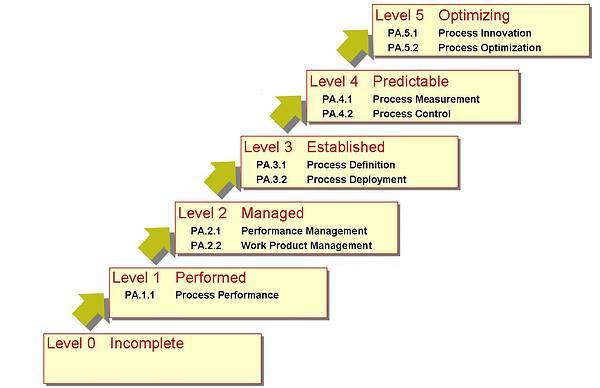
\includegraphics[scale=1,keepaspectratio]{SPICE.jpg}
\caption{SPICE}
\end{figure}
\FloatBarrier

Lo standard \textit{ISO/IEC 15504\ped{G}}, anche noto come \textit{SPICE\ped{G}} (Software Process Improvement and Capability Determination), definisce un modello di riferimento per la valutazione del livello di maturità dei processi. \\ 
Per l'esattezza sono previsti sei livelli di maturità, per i quali vengono definiti degli attributi che permettano di misurarla:
\begin{itemize}
\item\textbf{Level 0 - Incomplete process}: il processo non è implementato o non riesce a raggiungere i suoi obiettivi;
\item\textbf{Level 1 - Performed process}: il processo viene messo in atto e raggiunge i suoi scopi. Viene misurato tramite:
\begin{itemize}
\item\textbf{Process performance}: capacità di raggiungere i propri obiettivi e di ottenere risultati identificabili.
\end{itemize}
\item\textbf{Level 2 - Managed process}: il processo viene eseguito sulla base di obiettivi ben definiti. Viene misurato tramite:
\begin{itemize}
\item\textbf{Performance management}: capacità di elaborare un prodotto coerente con gli obiettivi attesi;
\item\textbf{Work product management}: capacità di elaborare un prodotto appropriatamente documentato, controllato e verificato.
\end{itemize}
\item\textbf{Level 3 - Established process}: il processo viene eseguito in base ai principi dell’ingegneria del software. Viene misurato tramite:
\begin{itemize}
\item\textbf{Process definition}: capacità di raggiungere i propri obiettivi aderendo agli standard;
\item\textbf{Process resource}: capacità di sfruttare risorse adeguate che gli permettano di essere attuato efficacemente.
\end{itemize}
\item\textbf{Level 4 - Predictable process}: Il processo è attuato all'interno di limiti ben definiti. Viene misurato tramite:
\begin{itemize}
\item\textbf{Process measurement}: capacità di utilizzare i risultati raggiunti e le misure ricavate durante l'esecuzione per garantire il raggiungimento dei traguardi definiti;
\item\textbf{Process control}: capacità di correggere o migliorare, se necessario,  le sue modalità di esecuzione, in seguito a controlli basati sulle misurazioni rilevate.
\end{itemize}
\item\textbf{Level 5 - Optimizing process}: Il processo è predicibile ed in grado di adattarsi per raggiungere obiettivi specifici e rilevanti. Viene misurato tramite:
\begin{itemize}
\item\textbf{Process change}: capacità di tenere sotto controllo tutti i cambiamenti strutturali e di esecuzione;
\item\textbf{Continuous improvement}: capacità di identificare
e implementare le modifiche effettuate, per garantire un miglioramento continuo nella realizzazione degli obiettivi fissati.
\end{itemize}
\end{itemize} 	

Ogni attributo definito precedentemente è misurabile e lo standard stabilisce
4 differenti livelli:
\begin{itemize}
\item\textbf{N}: non posseduto (0\% - 15\%);
\item\textbf{P}: parzialmente posseduto (16\% - 50\%);
\item\textbf{L}: largamente posseduto (51\% - 85\%);
\item\textbf{F}: completamente posseduto (86\% - 100\%).
\end{itemize}
\newpage
\section{ISO/IEC 9126}

\label{ISO/IEC 9126}
\begin{figure}[h]
\centering
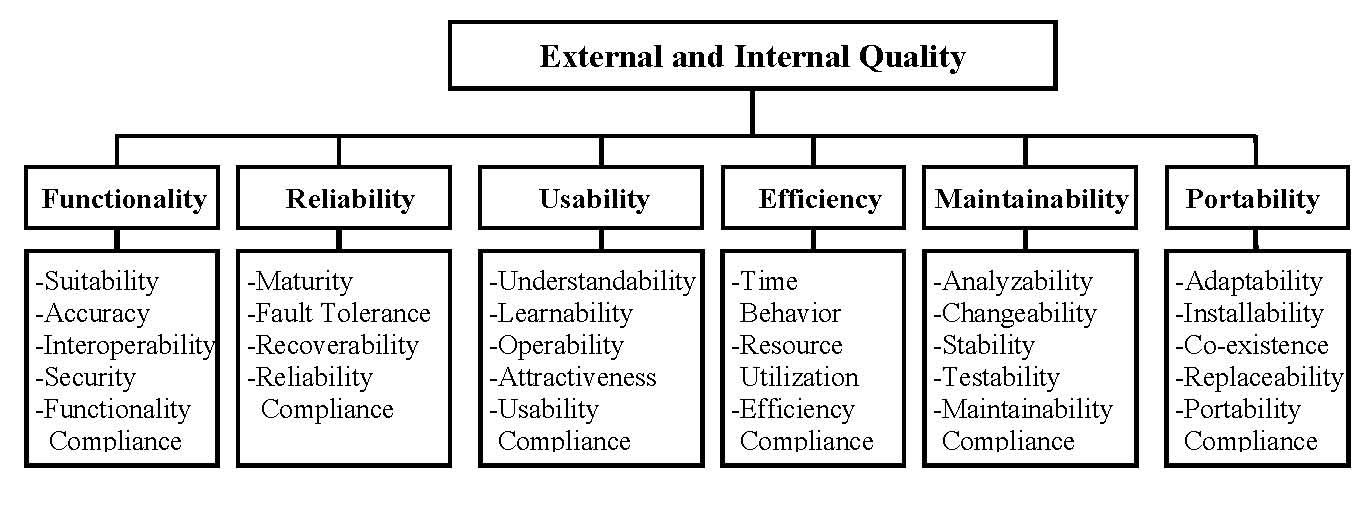
\includegraphics[scale=0.3,keepaspectratio]{9126.png}
\caption{ISO/IEC 9126}
\end{figure}
\FloatBarrier

Lo standard \textit{ISO/IEC 9126\ped{G}} è stato redatto con lo scopo di descrivere quali sono gli obiettivi qualitativi che deve avere un prodotto software. Questi vengono suddivisi in 3 aree tematiche diverse:
\begin{itemize}
\item\textbf{Qualità esterna}: rappresenta la qualità del software nel momento in cui esso viene eseguito e testato;
\item\textbf{Qualità interna}: rappresenta la qualità del software per quanto riguarda le sue caratteristiche implementative, durante le fasi di progettazione e codifica; 
\item\textbf{Qualità in uso}: rappresenta la qualità del software dal punto di vista del cliente che lo sta utilizzando.
\end{itemize}

Poiché non avremo la possibilità di testare la qualità in uso del prodotto, il \textit{team\ped{G}} ha deciso di concentrarsi solamente sulla qualità interna ed esterna. \\ Lo standard delinea sei macro-obbiettivi qualitativi, i quali sono suddivisi a loro volta in sotto caratteristiche specifiche:
\begin{itemize}
\item\textbf{Funzionalità}: capacità del prodotto di fornire tutte le funzioni che sono state individuate attraverso l'\textit{\AdR}:
\begin{itemize}
\item\textbf{Adeguatezza}: le funzionalità fornite devono essere conformi rispetto le aspettative;
\item\textbf{Accuratezza}: il prodotto deve fornire i risultati attesi, con il livello di precisione richiesto;
\item\textbf{Interoperabilità}: il prodotto deve poter interagire ed operare con uno o più sistemi specifici;
\item\textbf{Sicurezza}: il prodotto deve proteggere le informazioni e i dati da accessi e modifiche non autorizzati;
\item\textbf{Conformità di funzionalità}: il prodotto deve aderire a standard, regole e convenzioni inerenti alla funzionalità.
\end{itemize}
\item\textbf{Affidabilità}: capacità del prodotto software di svolgere correttamente le sue funzioni durante il suo utilizzo, anche nel caso in cui si presentino situazioni anomale:
\begin{itemize}
\item\textbf{Maturità}: il prodotto deve evitare che si verifichino malfunzionamenti o che vengano prodotti risultati non corretti;
\item\textbf{Tolleranza agli errori}: nel caso in cui si presentino degli errori, dovuti a guasti o ad un uso scorretto dell'applicativo, questi devono essere gestiti in modo da mantenere alto il livello di prestazione;
\item\textbf{Recuperabilità}: il prodotto deve essere in grado di ristabilire un
adeguato livello di prestazioni e di recuperare i dati rilevanti in seguito a errori o malfunzionamenti;
\item\textbf{Conformità di affidabilità}: il prodotto deve aderire a standard, regole e convenzioni inerenti all'affidabilità.
\end{itemize}
\item\textbf{Usabilità}: capacità del prodotto di essere facilmente comprensibile e attraente in ogni sua parte per qualsiasi utente che lo andrà ad utilizzare:
\begin{itemize}
\item\textbf{Comprensibilità}: l'utente deve essere in grado di riconoscerne le funzionalità offerte dal software e deve comprenderne le modalità di utilizzo per riuscire a raggiungere i risultati attesi;
\item\textbf{Apprendibilità}: deve essere data la possibilità all'utente di imparare ad utilizzare l'applicazione senza troppo impegno;
\item\textbf{Operabilità}: le funzionalità presenti devono essere coerenti con le aspettative dell'utente;
\item\textbf{Attrattiva}: il software deve essere piacevole per chi ne fa uso;
\item\textbf{Conformità di usabilità}: il prodotto deve aderire a standard, regole e convenzioni inerenti all'usabilità.
\end{itemize}
\item\textbf{Efficienza}: capacità di eseguire le funzionalità offerte dal software nel minor tempo possibile utilizzando al tempo stesso il minor numero di risorse possibili:
\begin{itemize}
\item\textbf{Comportamento rispetto al tempo}: per svolgere le sue funzioni il software deve fornire adeguati tempi di risposta ed elaborazione;
\item\textbf{Utilizzo delle risorse}: il software quando esegue le sue funzionalità deve utilizzare un appropriato numero e tipo di risorse;
\item\textbf{Conformità di efficienza}: il prodotto deve aderire a standard, regole e convenzioni inerenti all'efficienza.
\end{itemize}
\item\textbf{Manutenibilità}: capacità del prodotto di essere modificato, tramite correzioni, miglioramenti o adattamenti del software a cambiamenti negli ambienti, nei requisiti e nelle specifiche funzionali:
\begin{itemize}
\item\textbf{Analizzabilità}: il software deve consentire una rapida identificazione delle possibili cause di errori e malfunzionamenti;
\item\textbf{Modificabilità}: il prodotto originale deve permettere eventuali cambiamenti in alcune sue parti;
\item\textbf{Stabilità}: non devono insorgere effetti indesiderati in seguito a modifiche effettuate sul software;
\item\textbf{Testabilità}: il software deve poter essere facilmente testato per validare le modifiche effettuate;
\item\textbf{Conformità di manutenibilità}: il prodotto deve aderire a standard, regole e convenzioni inerenti alla manutenibilità.
\end{itemize}
\item\textbf{Portabilità}: capacità del software di poter essere utilizzato su diversi ambienti:
\begin{itemize}
\item\textbf{Adattabilità}: il prodotto deve adattarsi a tutti quegli ambienti di lavoro nei quali è stato previsto un suo utilizzo, senza dover apportare modifiche allo stesso;
\item\textbf{Installabilità}: il software deve poter essere installato in determinati ambienti di lavoro;
\item\textbf{Coesistenza}: il prodotto può coesistere in ambienti comuni
con altri software, condividendo risorse comuni;
\item\textbf{Sostituibilità}: l'applicativo deve poter sostituire un altro software che ha lo stesso scopo e lavora nel medesimo ambiente;
\item\textbf{Conformità di portabilità}: il prodotto deve aderire a standard, regole e convenzioni inerenti alla portabilità.
\end{itemize}
\end{itemize}	
\newpage
\section{Resoconto Attività di Verifica}
In questa sezione del documento vengono descritti e analizzati gli esiti delle attività di verifica svolte su tutti i documenti che vengono consegnati nelle varie revisioni di avanzamento del progetto.

\subsection{Revisione dei Requisiti}

\subsubsection{Tracciamento Casi d'Uso e Requisiti}
Il team ha deciso di utilizzare il software interno \textit{DocumentsDB} in modo da facilitare il tracciamento sia delle relazioni fra casi d'uso e requisiti, sia delle relazioni fra requisiti e fonti.

\subsubsection{Analisi Statica dei Documenti}
L'analisi dei documenti mediante \textit{walkthrough}\ped{G} ha portato all'individuazione di alcuni errori frequenti a partire dai quali è stata stilata una lista di controllo che è stata inserita all'interno dei "Processi Organizzativi" nelle \textit{Norme di Progetto}. Grazie a questa, sarà possibile applicare l'\textit{inspection}\ped{G} per le future attività di verifica.

\subsubsection{Esiti Verifiche Automatizzate}
Vengono qui riportati gli esiti delle verifiche automatizzate per il calcolo dell'indice \textit{Gulpease}\ped{G}, alle quali sono stati sottoposti tutti i documenti.
\begin{table}[h]
\begin{center}
\begin{tabular}{|c|c|c|c|}
\hline Documento & Indice Gulpease & Esito\\
\hline
\emph{Norme di Progetto} &  & Superato \\
\emph{Studio di Fattibilità} &  & Superato \\
\emph{Piano di Progetto} &  & Superato \\
\emph{Piano di Qualifica} &   & Superato \\
\emph{Analisi dei Requisiti} &  & Superato \\
\emph{Glossario} &  & Superato \\
\emph{Verbale} &  & Superato \\
\hline
\end{tabular}
\caption{Resoconto verifiche automatizzate - Revisione dei Requisiti}
\end{center}
\end{table}
\end{document}